\documentclass[preprint,11pt]{sigplanconf}

% The following \documentclass options may be useful:
% authoryear    To obtain author/year citation style instead of numeric.

\usepackage{amsmath}
\usepackage[T1]{fontenc}
\usepackage{graphicx}
\usepackage{color}

\newcommand{\fixme}[1]{\textcolor{red}{(FIXME: #1)}}

\begin{document}

\title{Verifying Interfaces in Ptolemy II}

\authorinfo{Ben Lickly}
           {University of California, Berkeley} {blickly@eecs.berkeley.edu}

\maketitle

\begin{abstract}
Interface theories provide useful machinery for proving properties of systems
and components, such as composition, refinement, shared refinement, and
feedback. One problem is that the details of the theories themselves are
ususally available only as a static specification, although many users
could benefit from being able to use an interfative environment for
experimenting with interface theories.

Here, we present just such a environement built on top of the Ptolemy~II
software framework. We have two primary groups of users in mind. The first are
system designers who are interested in leveraging interface theories to prove and test
properties of their models and systems.  The second are interface designers who
would like a maleable framework that allows them to experiment with new
interface theories, gaining an intuition for their theories by first
experimenting with new extensions and features.
\end{abstract}

\section{Introduction}
% FIXME: Flesh out this section
Component-based design allows large systems to be built more efficiently,
enforcing modularity that promotes reuse of existing components with
know behaviors, and allows diverse groups of developers create components
individually and be composed into a final system. 

Interface theories~\cite{interfaceTheories} specify what properties components
require of their environments, as well as how and when they can be abstracted,
composed, or refined. This often allows proving properties of the overall system
by combining properties of the individual components.

\subsection{Motivation}
Often, interface theories have their precise semantics captured only in the
English text of the works in which they are published. Rather than reading these
texts and performing the computations by hand, we would like to automate these
operations so that they can be checked (for some cases) by a computer. Since the
problem is undecidable in general, we accept having a partial algorithm that may
return "unknown."

One key question is that of interface composition.  In component based
verification, properties of the overall systems are proved by composing
properties of the components, and the interface theories tell us how to make
the compositions.

A typical example of where this type of tool would be useful would be in the
early stages of system specification. Different designers could specify certain
aspects of components to built that they would guarantee. This specification
could be done much more quickly than building even a prototype component, but
it would still be useful for specification. This tool would then be able to
check that these components can be composed. If it happens that this
requirement cannot be met, then the design must be reconsidered. This may point
to a fundamental design flaw, but it may also simply mean that some designers
must provide stronger guarantees of what their components will do.

For example, say we have two components, as well as some abstractions that
make up their interfaces, and be interested in the composition of those two
interfaces. One problem that might occur in this scenario is as follows: if the
interfaces of the original components are too abstract, then the interfaces
may not be composable. In this case, the developer may need to come up with a
more concrete interface, whose behavior is closer to the behavior of the
realized component. It would also be nice if we could algorithmically check
whether interfaces were composable, making this process faster and less
error-prone.

\section{Background/Related Work}
There are a variety of interface theories, beginning with the work of de Alfaro
and Henzinger~\cite{interfaceTheories}, and spawning several variants.  These
cast the view of components in a game-theoretic perspective, in terms of a game
between the component and its environment.  Here neither the component nor the
environment can control the other, but they may specify what they require of
the other.  The \emph{input assumptions} are the component's requirements of the
environment, which if violated make the environment lose.  The \emph{output
guarantees} are similarly the behavior that will cause the component to lose
if it does not satisfy.  We borrow there terms here.

Broy presents a theory of compositional refinement that deals with realations on
sequences produced by components~\cite{broy:1997:compositionalRefinement}. While
not billed as an interface theory, it shares many common elements, defining
notions of sequential composition, parallel compostion, and feedback. His theory
allows relations between inputs and outputs, but in order to do so it relates
sequences rather than values, and must also include notions of causality in order
to achieve feedback.

In addition, there are a variety of tools that attempt to combine static analysis
with concrete executions.
%
Larson and Austin propose an approach~\cite{larsonAustin:2003:coverageDetection} 
to checking security properties of programs that are input determined.  They do
this by abstracting the values of inputs and checking the desired properties on
these abstractions. This gives them predictive power by allowing concrete error
cases to flag error conditions that are produced by different input values on the
same execution path.

Gulavani et. al present a tool called Synergy~\cite{gulavani:synergy}, that
also combines testing with static analysis.  Synergy tries to prove program
properties by alternating between automated model checking of an abstraction of
the program with refinement of the abstractions based on test cases of
counterexamples.  The tool terminates if it is either able to prove the property
on an abstraction of the program, or it finds a concrete counterexample to the
program property.

In~\cite{relationalInterfaces}, Tripakis et. al. propose a relational type of
interface that can capture interactions between inputs and outputs.
This allows more complex behaviors to be captured, but it also means that
working with the interface theory can be more difficult.

Ptolemy II~\cite{ptII} is software system designed to facilitate experimentation
with actor-oriented modeling, and supports hierarchical compositions of
heterogeneous components.  Ptolemy~II has support for specifying interface
automata~\cite{Alfaro01interfaceautomata}, a type of interface that is specified
opertaionally, but this work is restricted to its own domain, and cannot be used
to annotate and check other actor models. Here, we aim to take a more denontatil
view of interfaces, concentrating on interfaces whose behavior is specified by
formulae. Ptolmey does support some types of semantic annotations at the actor
level, such as the causality interfaces presented
in~\cite{ZhouLee08_CausalityInterfacesForActorNetworks}, but this mechanism is
fairly specific to providing information about model time delays needed in the
PTIDES model of computation.

\section{Approach} %FIXME: Beef this up?
Here, we aim to build a system for automatically checking the satisfiability
of such interfaces and to aid in composing them. We choose to base our work on
Ptolemy II since it already has a large library of actor models, and provides a
flexible platform for experimentation.

We see our current problem, and the resulting solution, as affecting two
parties:
1. model designers, who would like to use interface theories verify properties
of their models; and
2. theory designers, who would like to develop new interface theories.
%
Any solution must keep both parties in mind, making sure that properties
can be specified intuitively and necessary features for property proving are
provided, as well as abstracting out details of the individual interface theory
so that it can be changed later.

\subsection{Definitions}
We define a deterministic interface to be one for which the outputs are
uniquely determined by the inputs (and the current state, if stateful) for all
valid inputs.
Even though most of our real components behave deterministically, our
interfaces are in general abstractions of this behavior, and thus they are
often not deterministic.
Informally, we can discuss one interface being more deterministic (or more
abstract) than another.

An interface $A=(X,Y,\phi_A)$ is \emph{more deterministic} than interface
$B=(X,Y,\phi_B)$, if
\[
\phi_B \implies \phi_A \wedge \phi_A \not\implies \phi_B
\]
If we view the contract as simply specifying a relation between the inputs and
the outputs, $R(\phi) \subseteq X \times Y$, then A being more deterministic
than B simply means that $R(\phi_A) \subset R(\phi_B)$

% We can get the input assumptions from a relational interface by
% projecting the relation onto only the input variables.  In terms of
% the logical formula, this can be achieved by simply extistentally quantifying
% out the output variables.  We write the input assumptions of contract $\phi$ as
% $in(\phi)$.

\subsection{Examples}
Let us consider a component that performs a division operation.  In order to
function, it requires that its environment not provide a zero-valued input as
its denominator, as that would be a divide-by-zero opertaion. In traditional
interface theories, where interface of a component is specified by separate
input assumptions and output guarantees, the only piece of information about
the behavior of a component is its input assumption, namely that the
denominator input must be non-zero. In Ptolemy, we might annotate these
restrictions as shown in Figure~\ref{fig:dividerOld}.

\begin{figure}[htbp]
\centering
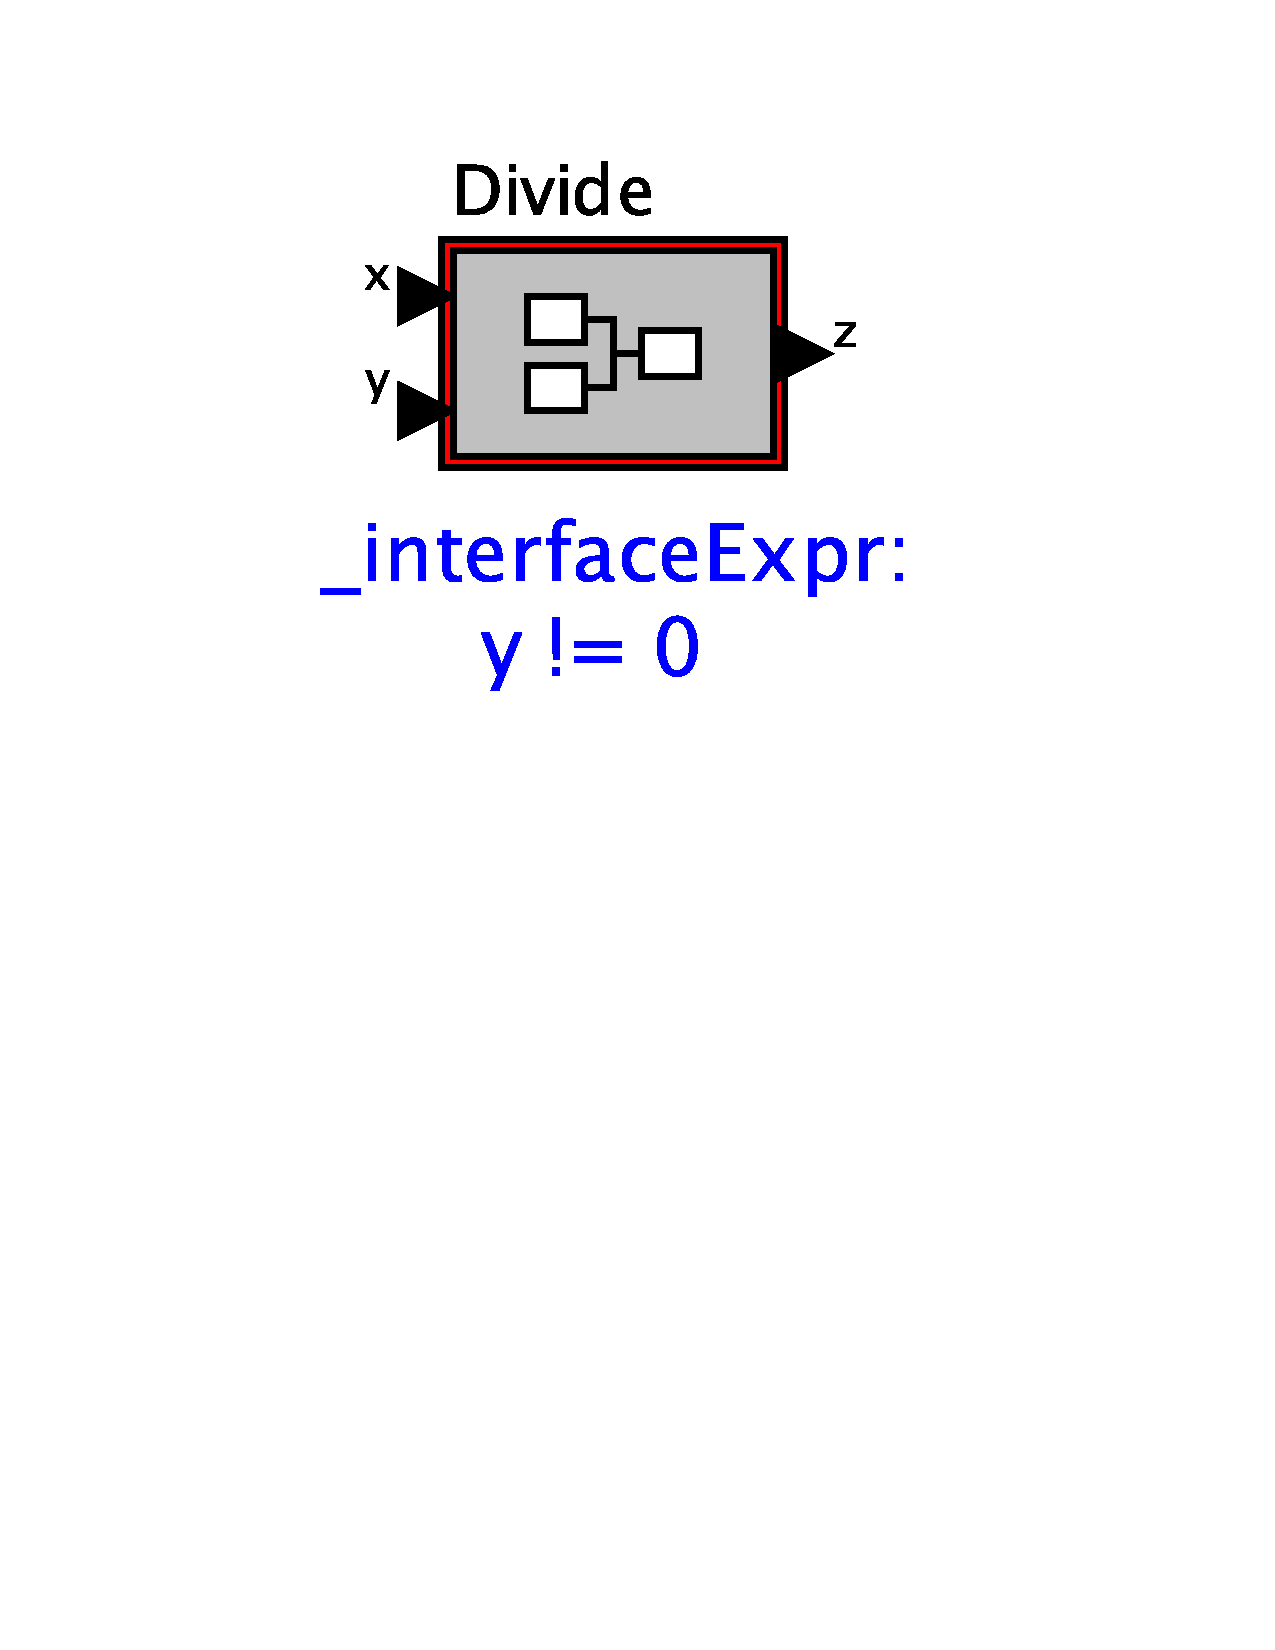
\includegraphics[scale=0.55]{figs/divideSimplest}
\caption{A non-realtional interface of a divider actor.}
\label{fig:dividerOld}
\end{figure}
\cite{ptII}
In a relational interface theory, however, we can express interfaces that are
more deterministic than this.  In fact, since this is a completely
deterministic component, whose behavior is uniquely determined by its (valid)
inputs, we can specify a completely deterministic interface.  We have shown how
this may look in Ptolemy in Figure~\ref{fig:dividerNew}, but it simply says
that the denominator must be non-zero, and the output is the quotient of the
numerator and the denominator.

\begin{figure}[htbp]
\centering
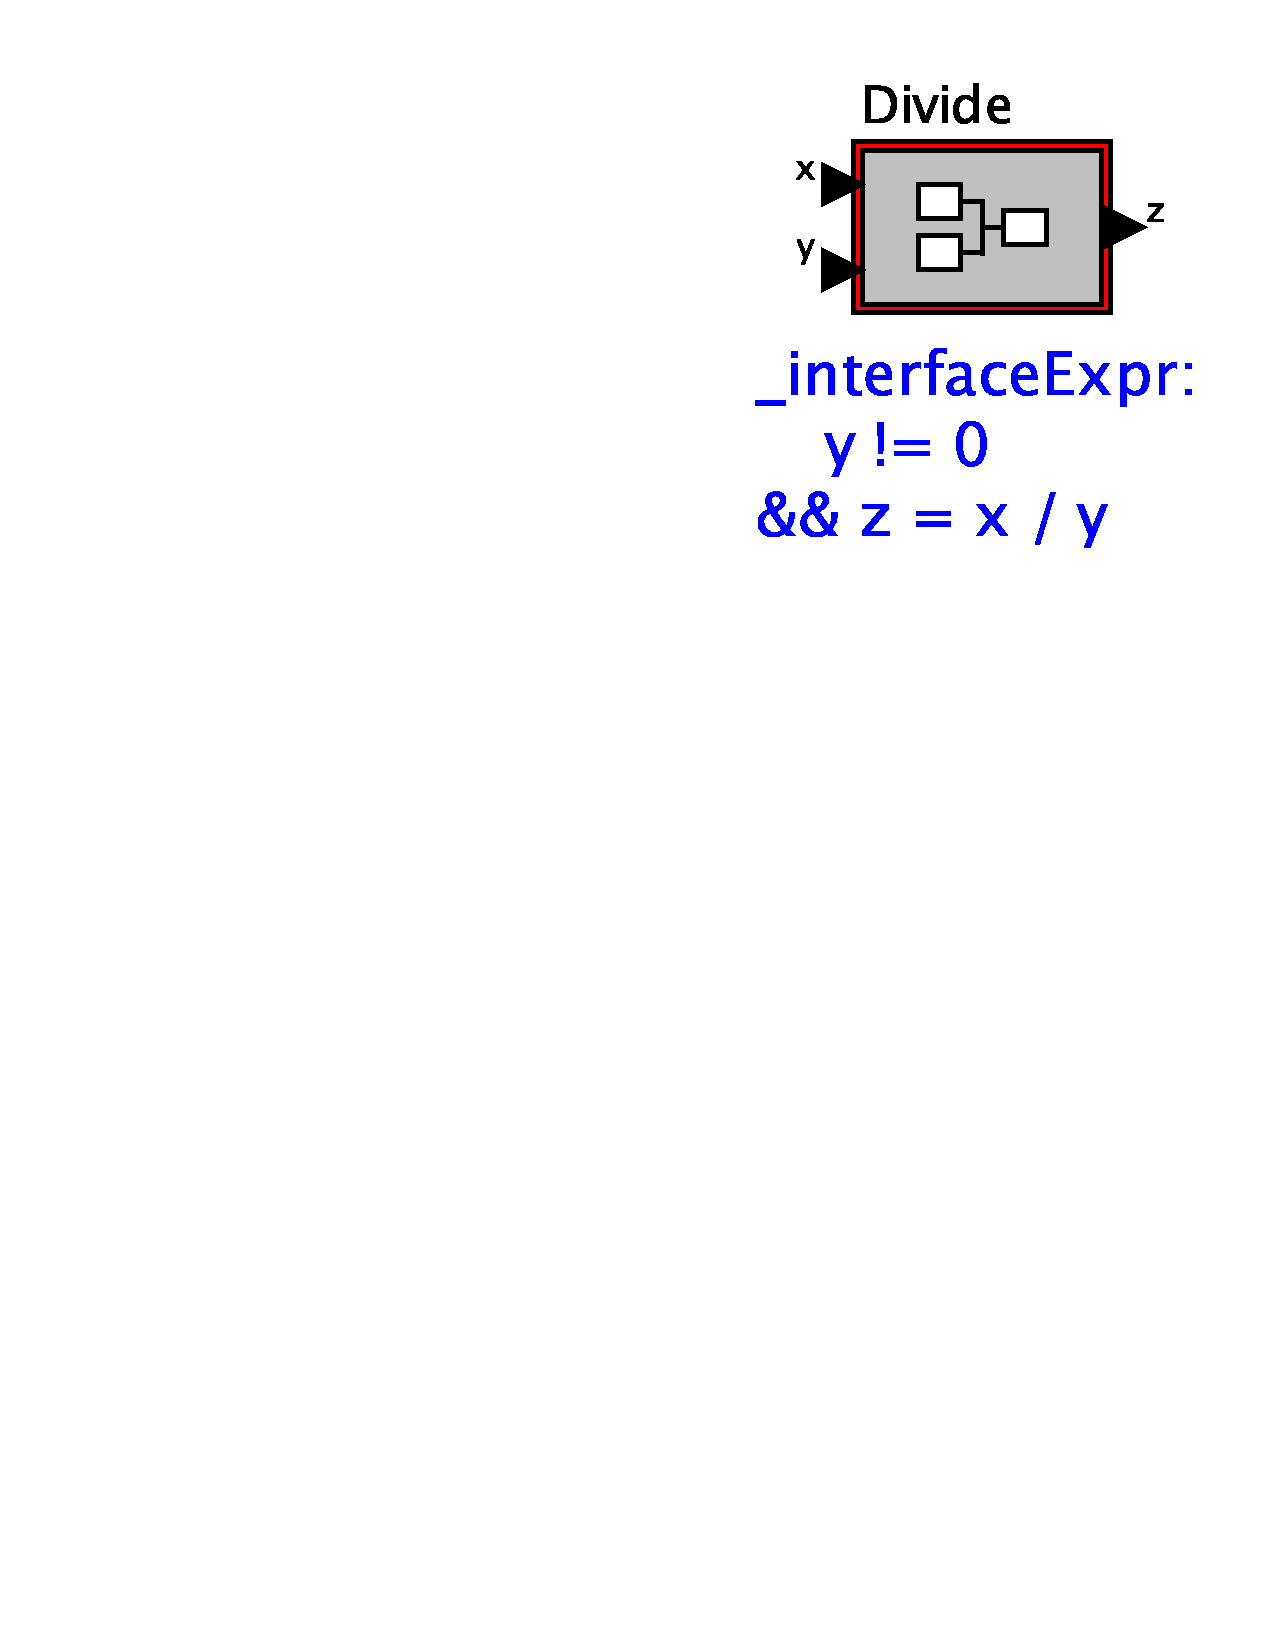
\includegraphics[scale=0.6]{figs/Divide2} 
\caption{A relational interface of a divider actor.}
\label{fig:dividerNew}
\end{figure}

Notice that if we want to recover the input assumptions from a relational
interface, we can simply project the contract onto the input variables by
quantifying out the outputs. In this case, the input assumptions are 
\[
\exists z : y \ne 0 \wedge z = x / y 
\]
This is equivalent to simply $y \ne 0$, which was exactly the input assumption
that we had previously.

In general, for a relational contract $\phi$, we will define the \emph{input
assumptions} of $\phi$, $in(\phi)$ to be the results of this projection onto
the input variables.

\section{Solution}
Since there is ongoing research on creating industrial-grade SMT solvers,
we elect to integrate an existing solver rather than create one from scratch.
Our approach leverages the Yices\cite{yices} SMT solver, interfacing it to
work in the Ptolemy II modeling framework.

We create a new Ptolemy~II director, called the
\texttt{InterfaceCheckerDirector}, which checks the validity of the interfaces of
the actors in a model. We allow each actor in the model to be annotated with a
parameter to specify its interface. Here we supporting both native Ptolemy~II
expressions, which have a C-like syntax, and LISP-style string expressions in the
Yices input language. The Ptolemy expressions must be boolean valued, with a true
value meaning the interface is satisfied, and they are searched for by looking
for parameters of actors named $\_interfaceExpr$. The Yices inputs language
interfaces require string-valued parameters names $\_interfaceStr$, and allow
richer expressions to be used. This is because the Yices input language supports
quantifiers, which are absent in the Ptolemy expression language.

The details of the interface theory itself are encapsulated in the
\texttt{RelationalInterface} class, allowing for different interface theories
to be added later.  This class defines the methods for composing interfaces
with each other in different types of ways, adding feedback, and exporting the
interface definition to a format that Yices can check. In cases where these
compositions or feedbacks are not possible, the interface theory can throw an
exception.
%
In this intial implementation, only the relational interface theory
of~\cite{relationalInterfaces} is supported, but we hope to construct and
experiment with many variations and new theories using this infrastructure.

\subsection{Supported Operations}
One of the most critical opertaions that we want to support is that of
inferring the composition of components.  Ptolemy II includes a special type
of actor whose definition is a composition of other actors, the
\texttt{CompositeActor}. We can then exhibit our different types of inferrence
by simply specifying them as fallback options for determining the interfaces of
\texttt{CompositeActor}s that do not have interface annotations.

Broadly, there are three types of composition in which we are interested.
%
The simplest type of composition is parallel composition.  When we want to
compose two interfaces in parallel, such as the independent components of the
Doubler and Halver in Figure~\ref{fig:parallelComp}, then all we need to do is
combine the two component interfaces.  Formally, the inferred contract is simply
the conjuntion of the component constracts.

\begin{figure}[htbp]
\centering
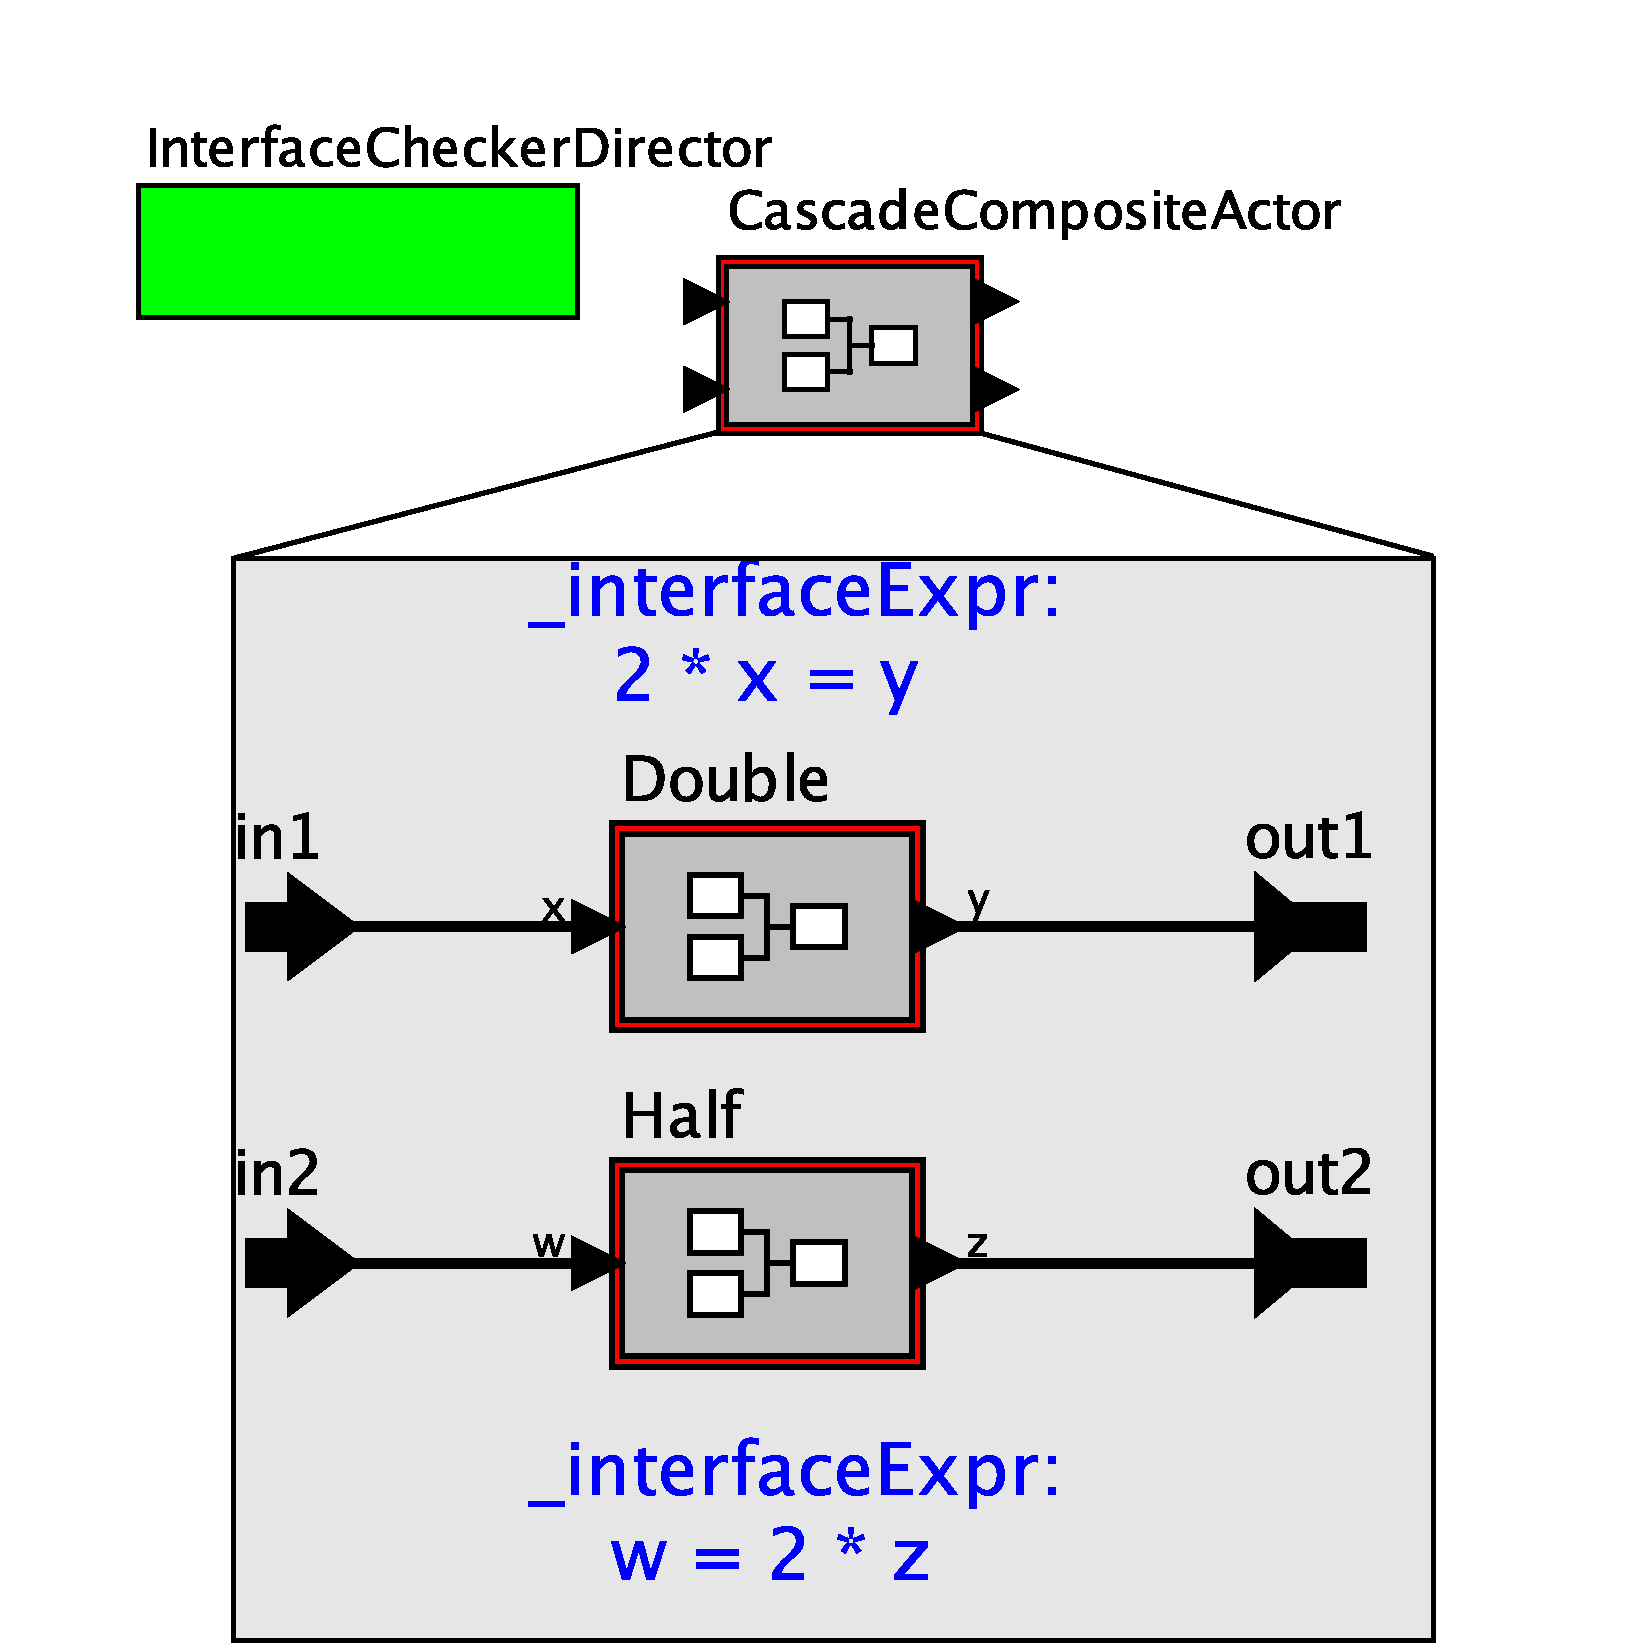
\includegraphics[width=\columnwidth]{figs/parallelComp}
\caption{A composite actor formed by the parallel composition of two contained
actors.}
\label{fig:parallelComp}
\end{figure}

A slightly more complex case arises when there is a feedback connection from an
output of a component back to its input. There is a resriction on when this can
happen, since some types of feedback, like connecting a not gate to itself, do
not make sense. In the theory used here, only feedback connections in which the
input port is unrestricted are allowed. We can check this condition
syntactically, without needing to use the SMT solver.  When a feedback
connection is allowed, such as in Figure~\ref{fig:feedbackComp}, the inferred
contract simply needs to add a constraint that the connected ports are equal.
In our example, when the output port $z$ is connected to the input port $x$, we
simply conjoin the original contract with the constraint $x=z$.

\begin{figure}[htbp]
\centering
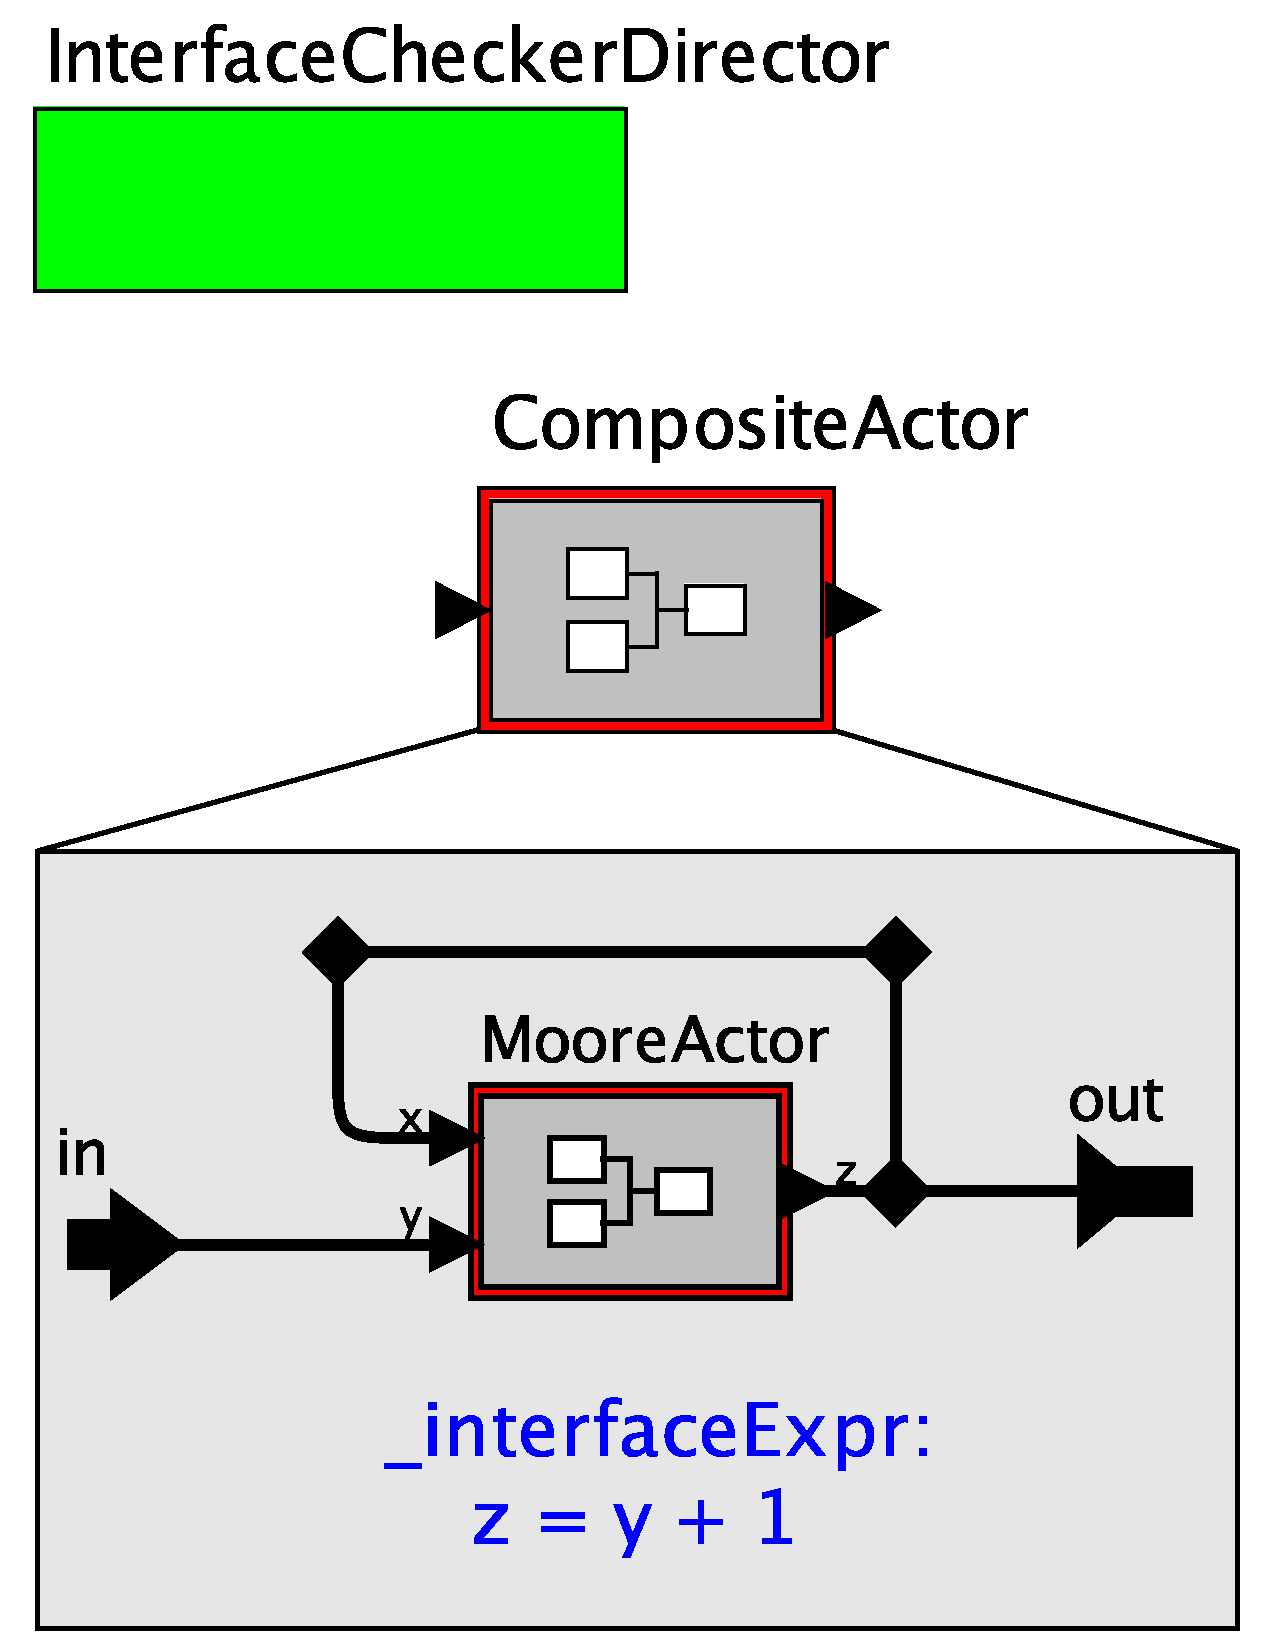
\includegraphics[width=\columnwidth]{figs/feedbackComp}
\caption{A composite actor formed by adding feedback to its contained actor.}
\label{fig:feedbackComp}
\end{figure}

The most complicated case arises when we have cascading composition, or
composition in which the outputs of one interface are the inputs to the next.
In order to make these compositions, we need to first ensure that the output of
the first interface will always be a valid input to the second interface.  We
treat the component interfaces as black boxed over which we have no direct
control.  The only way that we can affect the components is through restricting
the valid inputs to the composite interface.
%
For example, in the case of Figure~\ref{fig:cascadeComp}, we need to ensure
that the output of $LeftActor$ is valid input to $RightActor$.  Since our
interface of $LeftActor$ makes no guarantees about what output it will produce
when the input is anything other than 1, it could potentially produce 0. Thus,
we must disallow any input other than 1, and our composite interface must have
the input assumption that $in = 1$.

\begin{figure}[htbp]
\centering
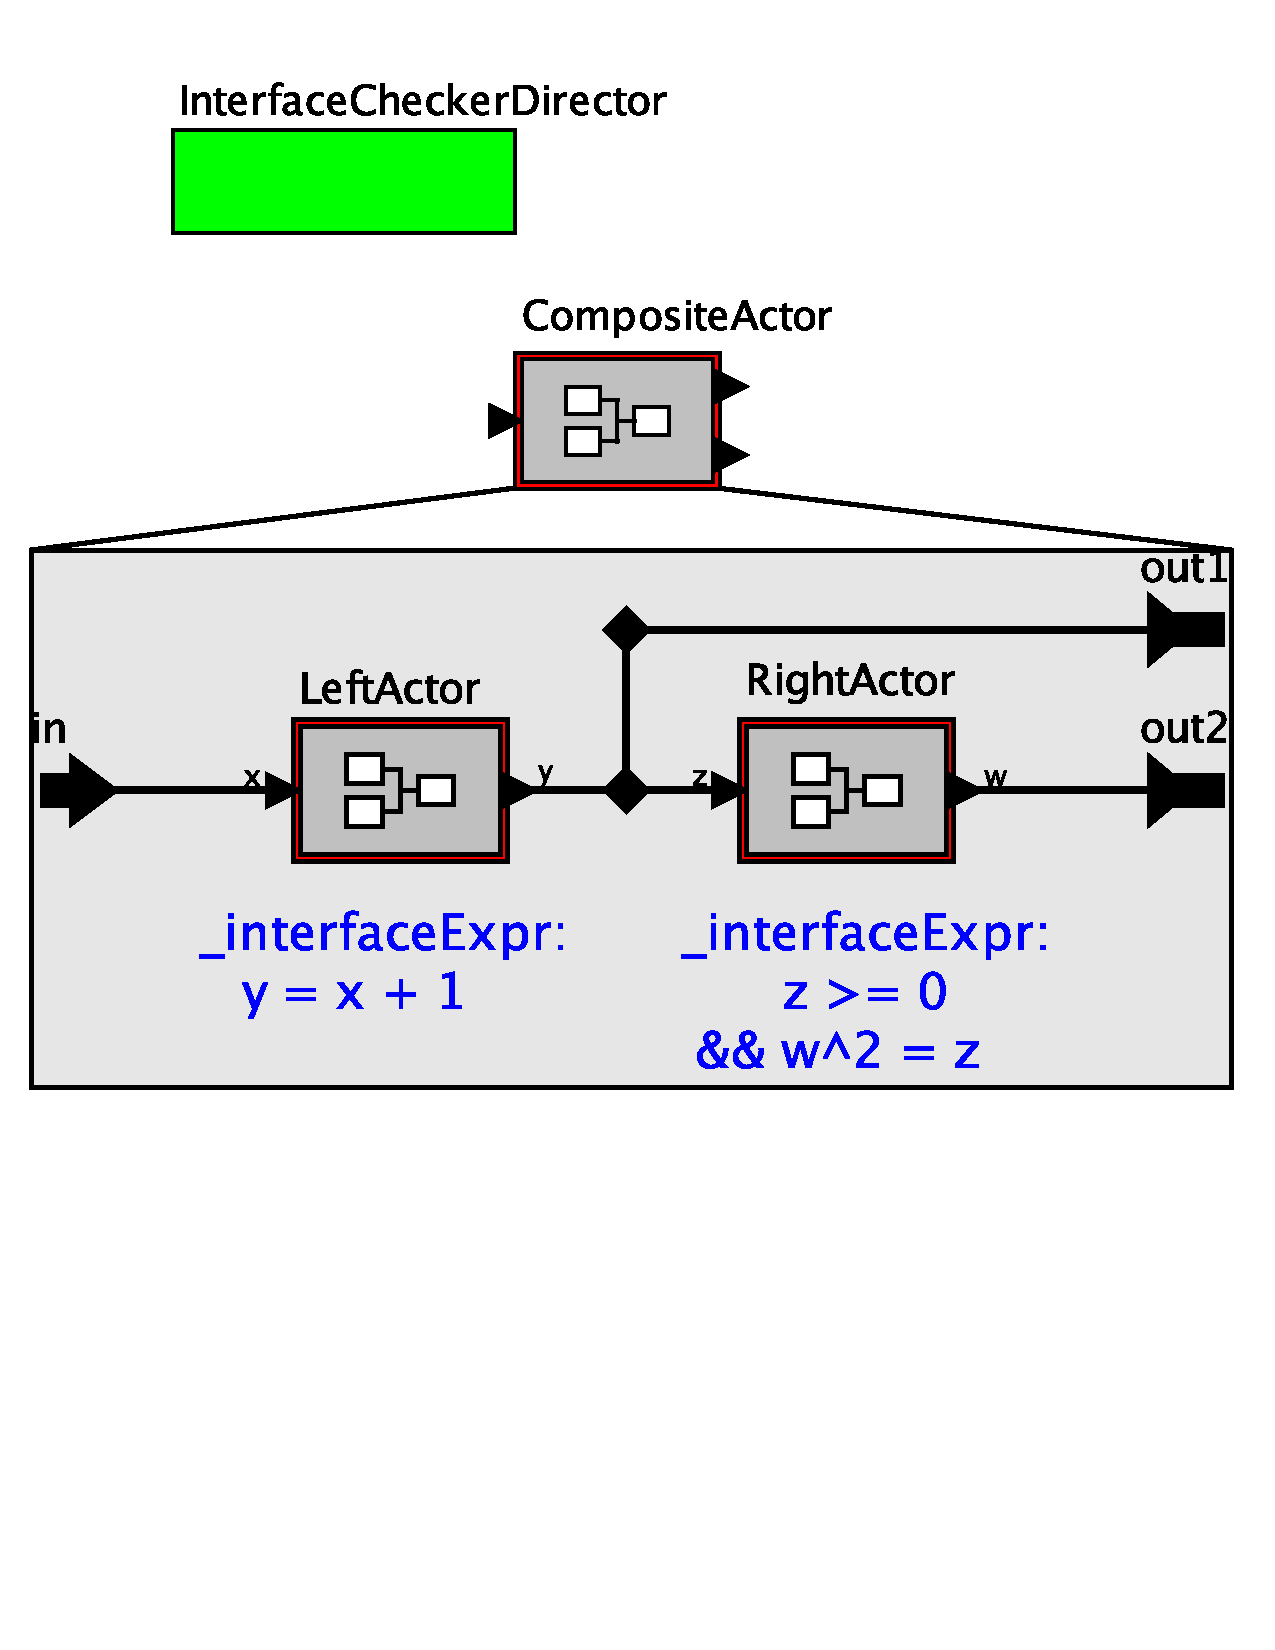
\includegraphics[width=\columnwidth]{figs/cascadeComp} 
\caption{A composite actor formed by the cascade composition of two contained
actors.}
\label{fig:cascadeComp}
\end{figure}

Formally, the composition interface is defined in the following way. In order
to cascade compose the output of interface $I_1$ into the input of interface
$I_2$, we get the following composite interface contract.
\[
\phi_1 \wedge \phi_2 \wedge \theta \wedge \forall Y: \Phi
\]
where $\phi_1$ and $\phi_2$ are the contracts of the components, $\theta$ are
the constraints that the connected outputs and inputs are equal, $Y$ are all
the ports other than the inputs to the composite interface, and $\Phi$ is the
restriction on the inputs of the composite interface to make the composition valid.
$\Phi$ is given as follows:
\[
(\phi_1 \wedge \theta) \implies in(\phi_2)
\]
This simply means that for all possible responses to the inputs that meet the
contract of the first interface and the connections, the input assumptions to
the second interface are met.


\subsection{Usage Examples}
This section chronicles possible use cases of the new interface analysis from a
user's point of view.
%FIXME: Make me flow better!

In the first example, a user wants to compose two components, the first of
which takes the absolute value of its input, and the second of which takes the
inverse of its input. In order to guarantee that the components have a valid
composition, the user must first check that the interfaces are composable.
In this example, the components themselves can be connected sucessfully, as
long as we restrict the inputs to the composition to be non-zero.  We will see,
however, that what we can prove depends on choosing the right abstractions.
Since interfaces are used to prove safety properties of the system, any
abstractions must be overapproximations.

\subsubsection{Interface Error}
\begin{figure}[htbp]
\centering
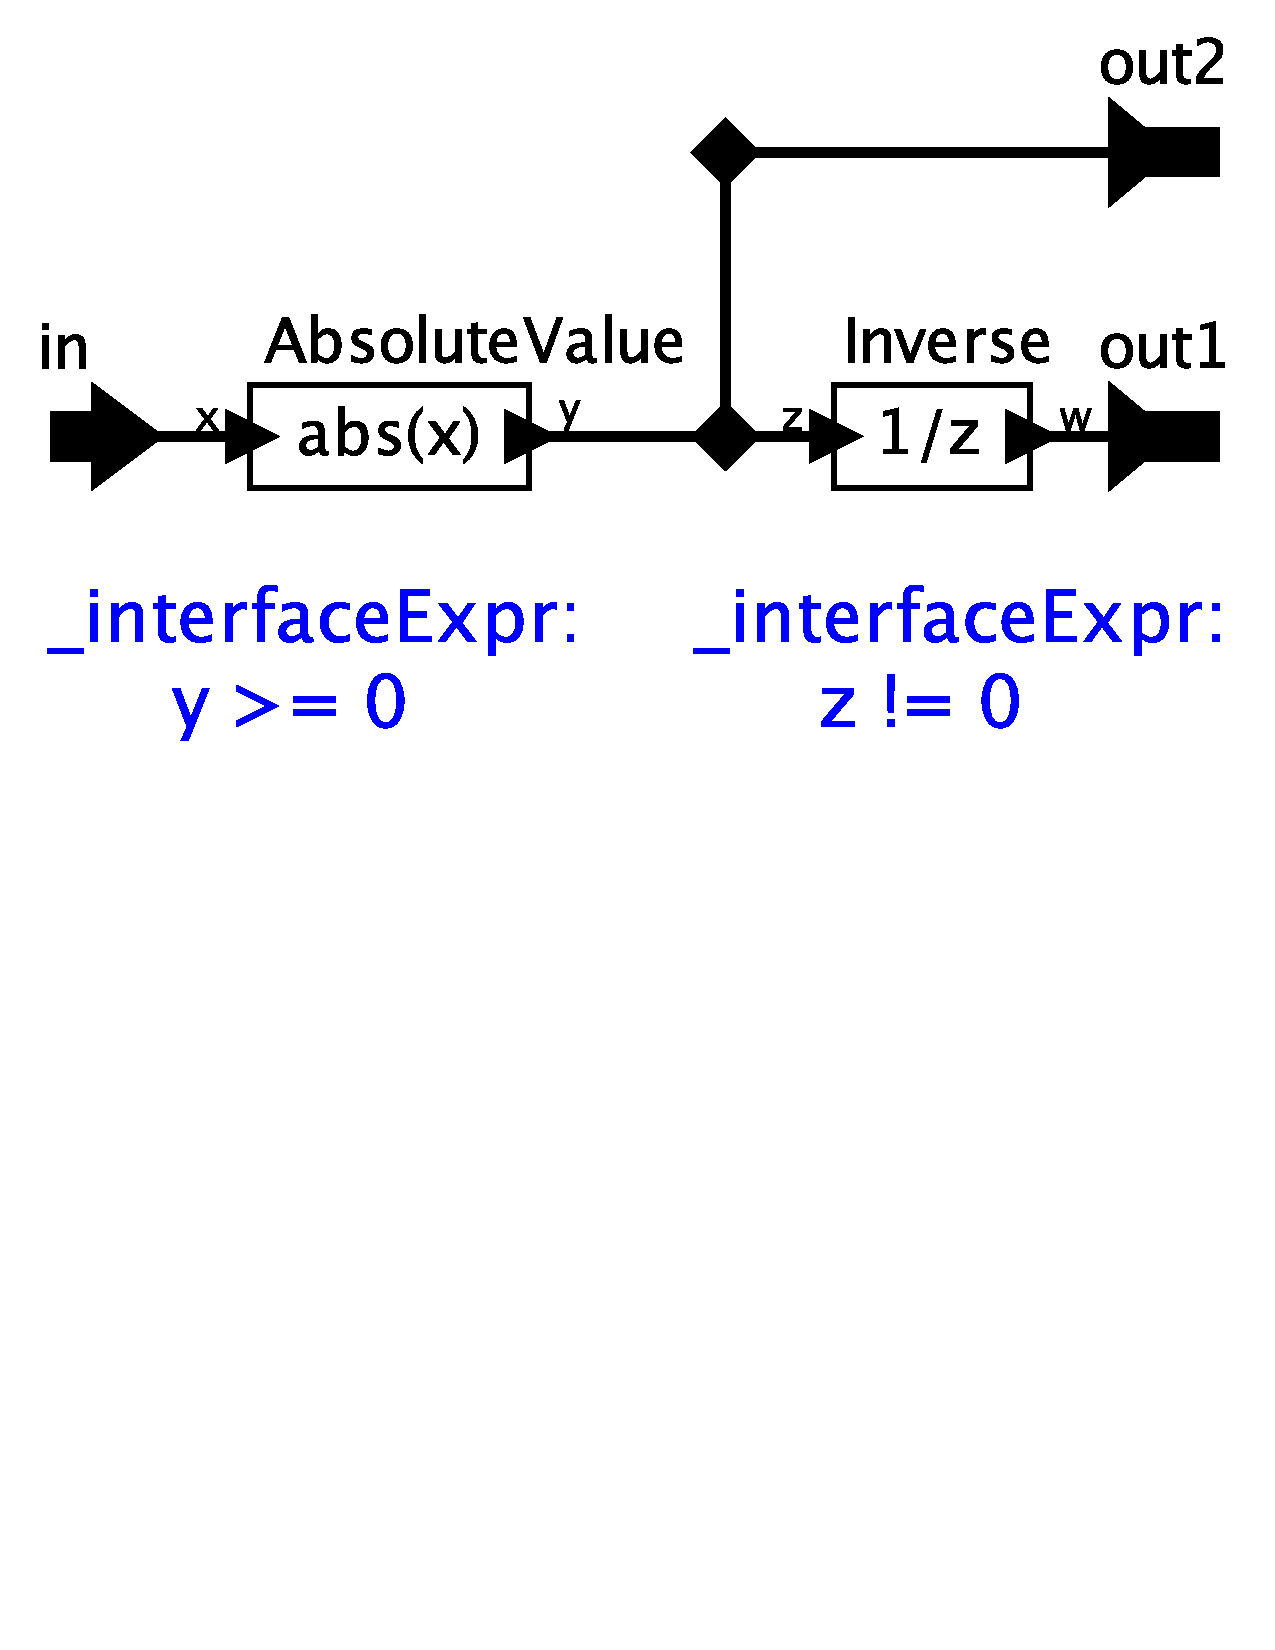
\includegraphics[width=\columnwidth]{figs/absoluteError}
\caption{An error in interface specification.}
\label{fig:absoluteError}
\end{figure}

In the first attempt at choosing interface abstractions, shown in
Figure~\ref{fig:absoluteError}, the user choses the contract
\[
y \ge 0
\]
for the absolute value.  This only guarantees that the output will be
non-negative, regardless of the input. This is an overapproximation of
absolute value, since it doesn't take into account the input to the actor.
%
For the inverter, the user choses the contract
\[
x \ne 0
\]
to capture the restriction that we cannot divide by zero.
Since this contract does not specify the output value, it too is an abstraction
that overapproximates.

In this case, when we check our interfaces our tool will tell us that the
resulting composition interface has an unsatisfiable contract, showing that the
interface is not valid. Intuitively, this is because there is no input to the
first component's interface such that we can guarantee its output will not be
zero. Since these interfaces do not compose, we need to make them more concrete.

\begin{figure}[htbp]
\centering
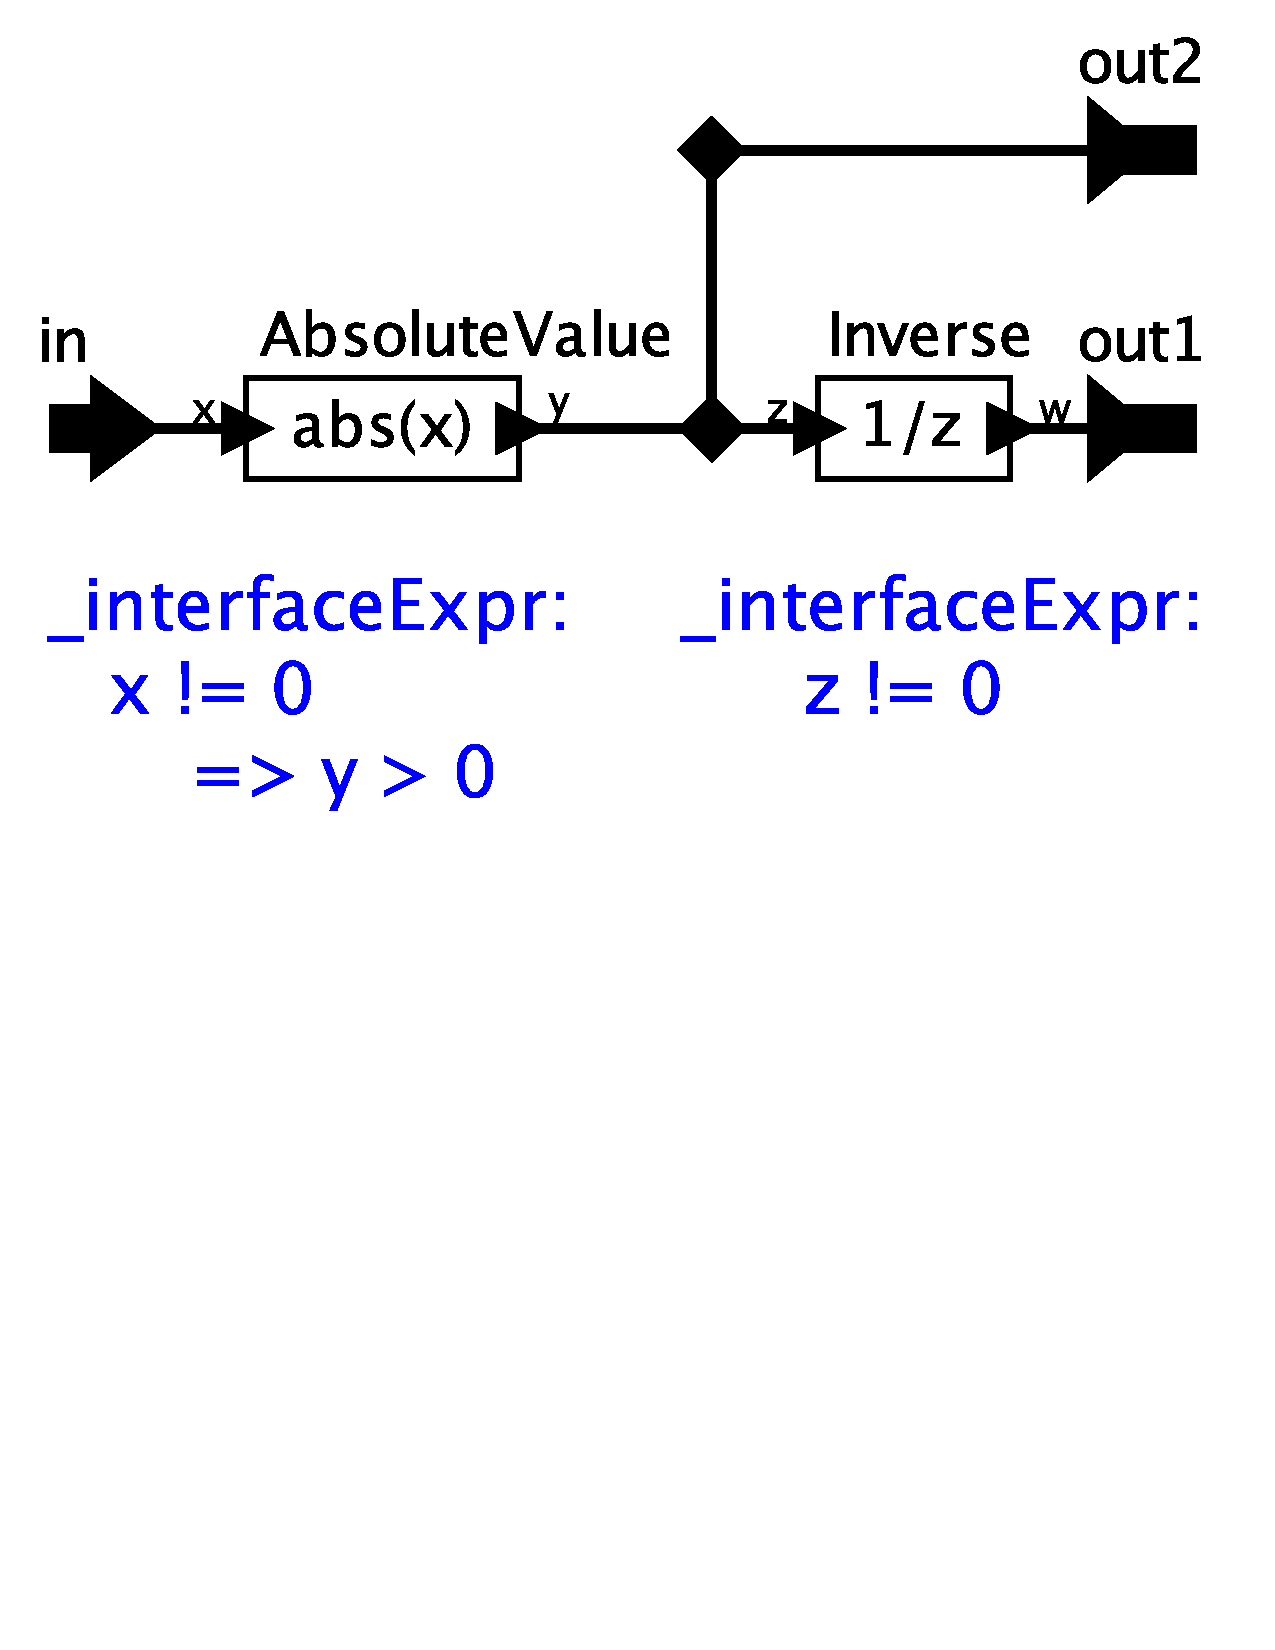
\includegraphics[width=\columnwidth]{figs/absoluteCorrected}
\caption{A fixed interface specification.}
\label{fig:absoluteCorrected}
\end{figure}

A second attempt at defining the component interfaces for this same model is
given in Figure~\ref{fig:absoluteCorrected}.
Here, the interface of the inverter is unchanged,
but the interface for the absolute value is made more deterministic, changing
its contract to
\[
x \ne 0 \implies y > 0 .
\]
% P.S. Let's try an example with \[ x \ge 0 \implies y = x\] or even 
% \[ x \ge 0 \implies y = x \wedge x < 0 \implies y = -x\]
This interface is still an abtraction, it does not specify exactly what
the result of any input is, or even mention what the absolute value of zero is.
All it says is that the absolute values of non-zero inputs are positive.
This is concrete enough, however, to define the interface of the composite.  In
particular, we can guarantee that given a non-zero value to the composite, we
will avoid an error within the component, which is exactly correct.

\subsubsection{Component Error} \label{sec:componentError}
\begin{figure}[htbp]
\centering
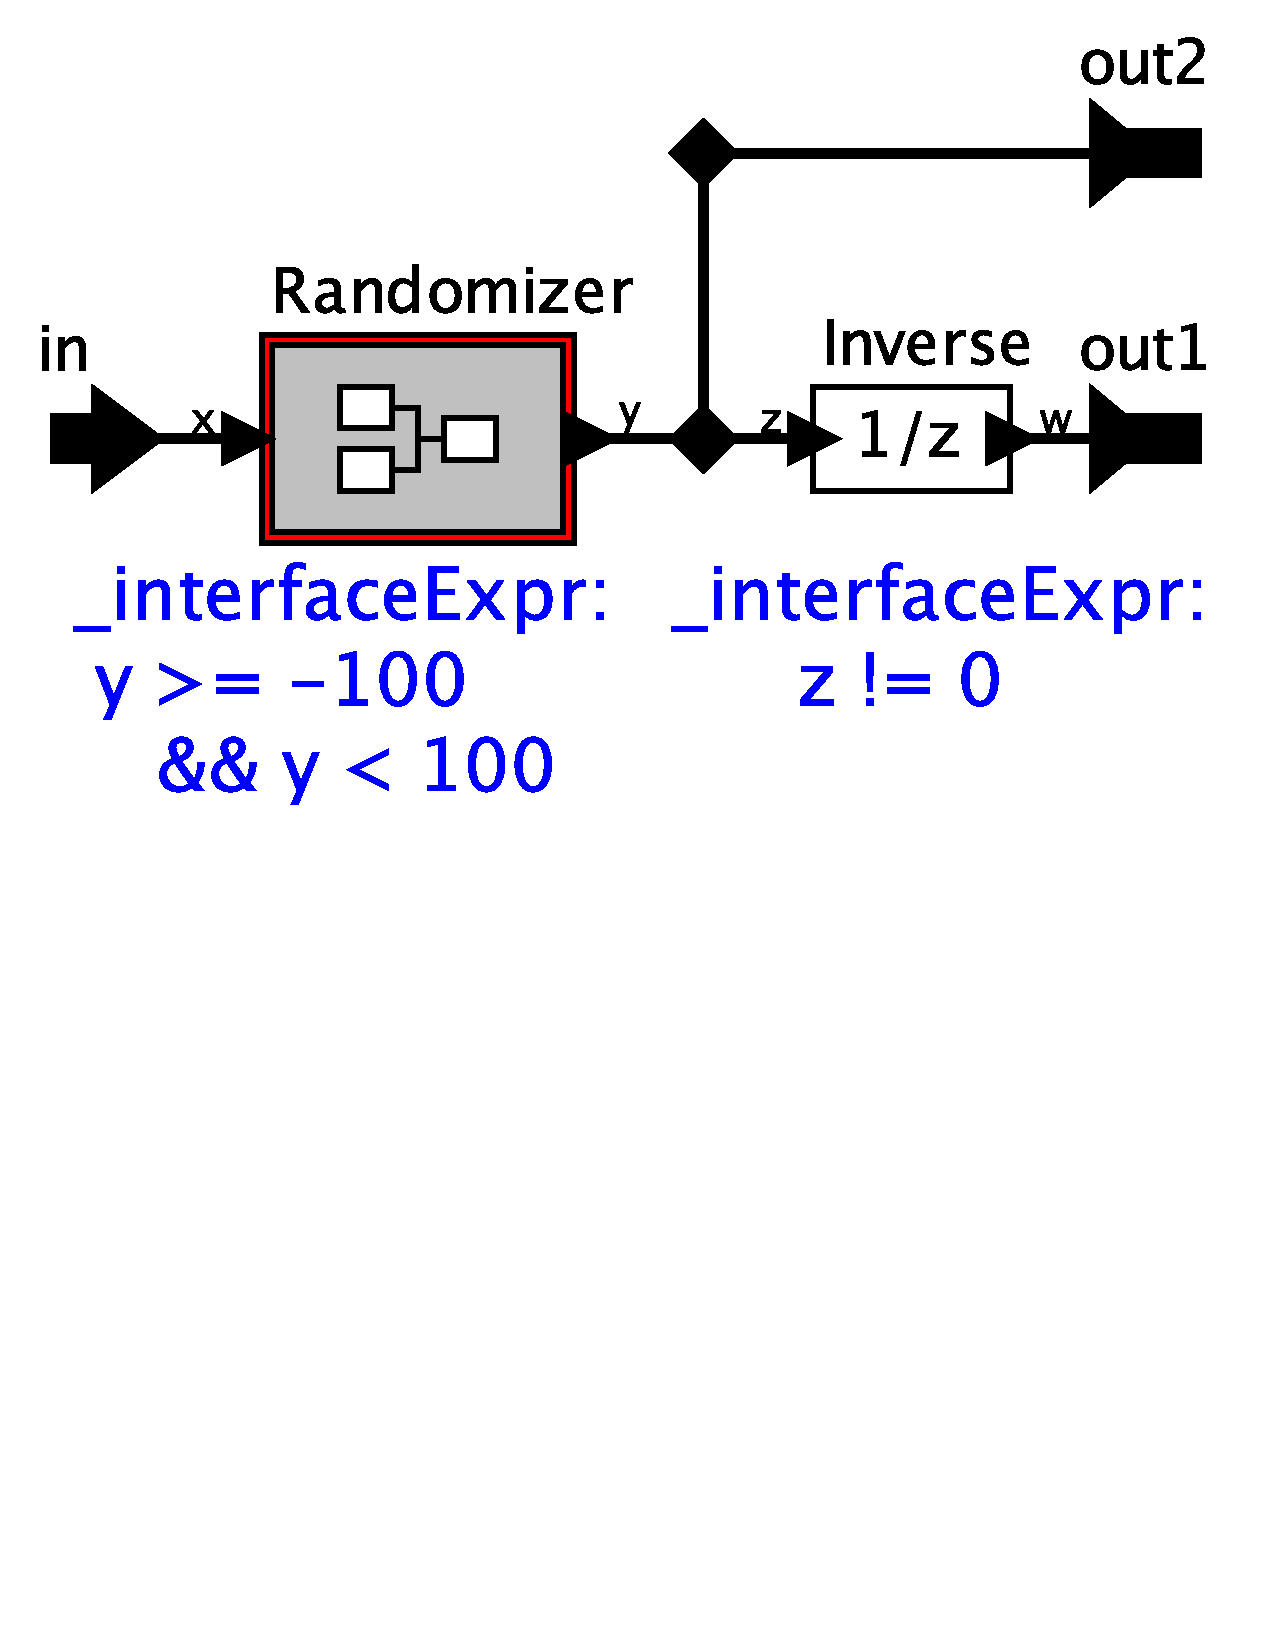
\includegraphics[width=\columnwidth]{figs/Randomizer}
\caption{An error in component composition.}
\label{fig:randomError}
\end{figure}

Consider another example in which the first component produces a random value
in the range $[-100, 100)$, and the second component is the same as
before.
The most deterministic valid constraint that the user can use for the first
component would be
\[
y \ge -100 \wedge y < 100
\]

In this case, running our tool will tell us that these components cannot be
composed.
This time, however, this is not caused by the interfaces being too abstract;
in fact, they are maximally deterministic.
The reason why we cannot compose these interfaces is that these components
cannot be safely composed.
Even though testing may not produce the error in a given run, there is always
the possibility that this first component will produce a zero-valued output. 
Since we are not allowed to look inside or change the components we are given,
the only response our tool can give is to disallow such composition.

\section{Ongoing work}
As a general infrastructure, there are many possible extensions.
One would be the addition of run-time checks to test that the values produced
by the implementation conform to the interfaces. This could be a check of both
the implementations and the interfaces. Interestingly, these checks could even
have predictive power. As an example, consider Figure~\ref{fig:randomJitter}.
Here, the first component adds a value to its input that is randomly chosen
from the range $[-100,100)$. Since there is non-determinism in the component,
the given interface, $y \ge x-100 \wedge y < x+100$, is as deterministic as
possible. Unlike the totally random component from Figure~\ref{fig:randomError}, these
components can be validly composed by restricting the acceptable inputs $x$
that can be provided to the composite. In isolation, static analysis on this
component will declare it to be error-free. \begin{figure}[htbp]
\centering
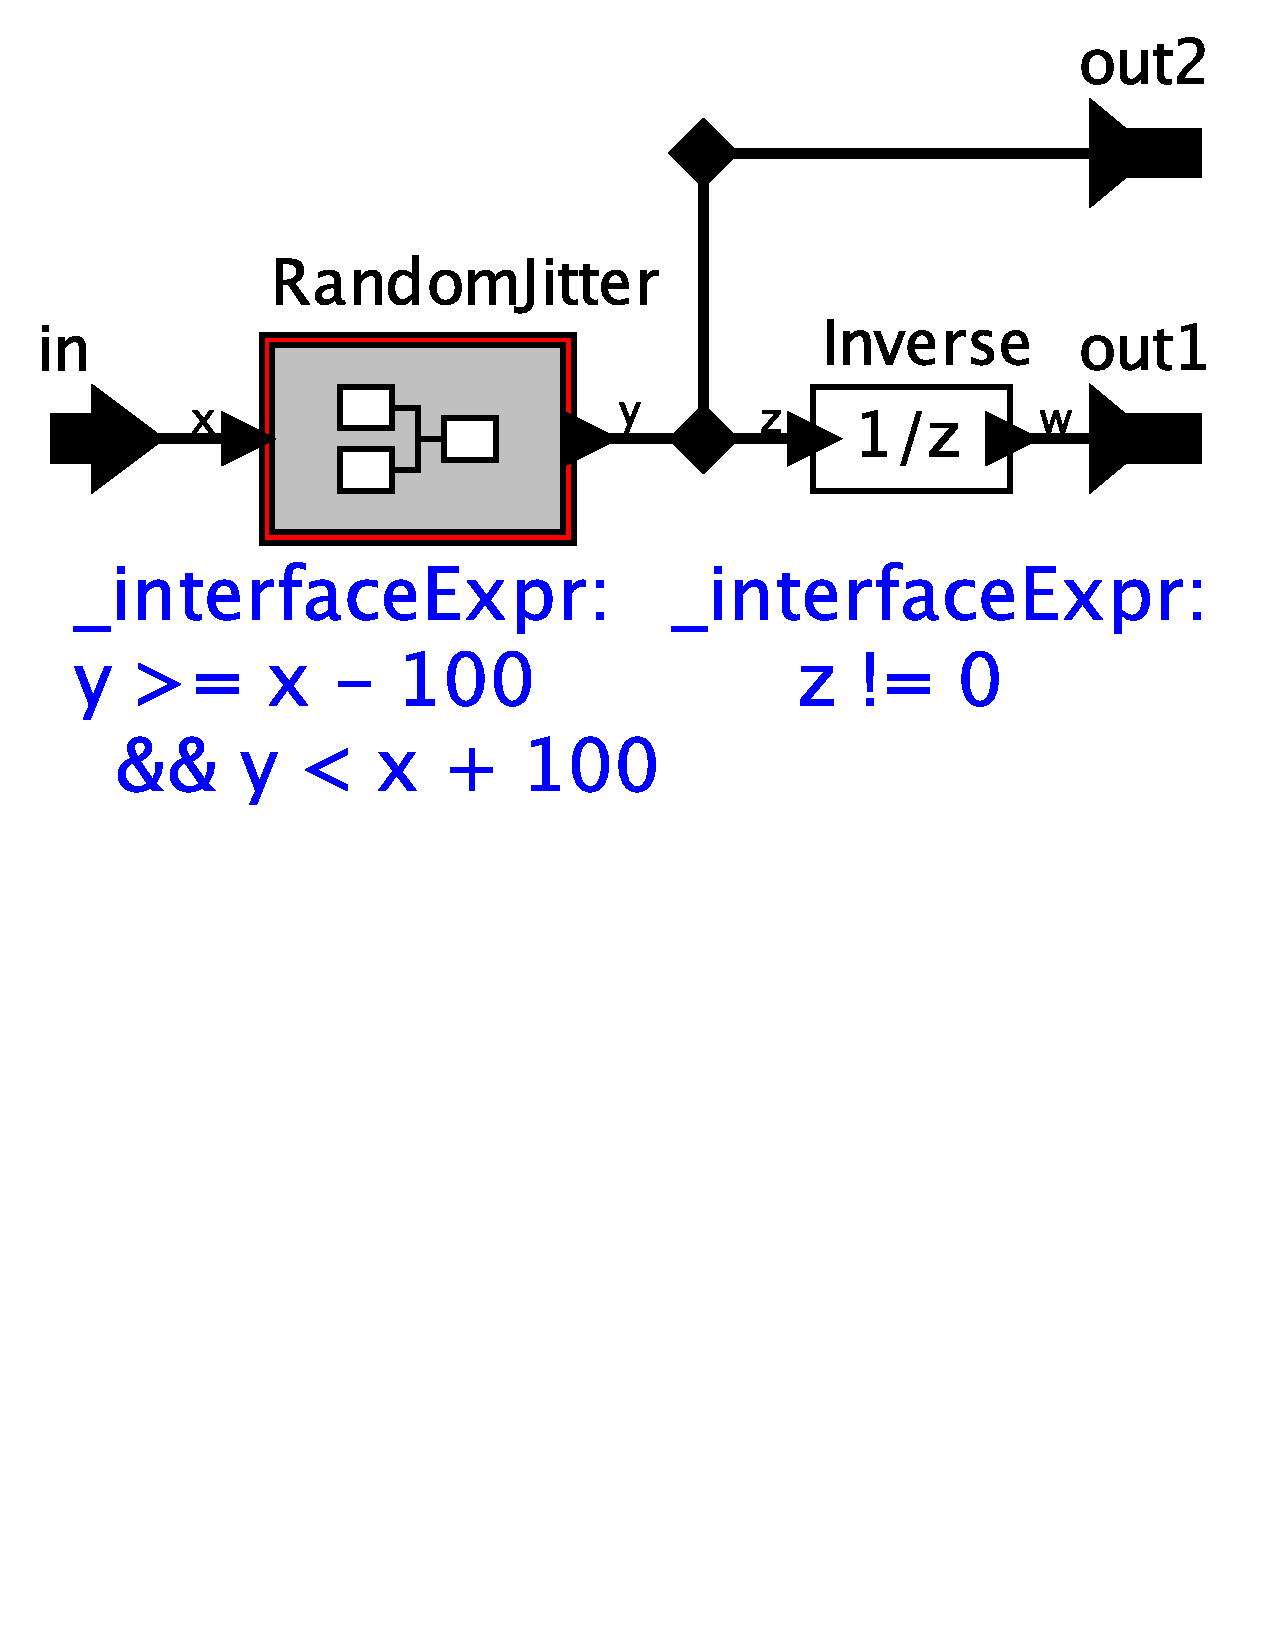
\includegraphics[width=\columnwidth]{figs/randomJitter}
\caption{A component with an error that may not show up through testing.}
\label{fig:randomJitter}
\end{figure}
Imagine that we had test cases that ran this code with an input of $42$.
This would be an erroneous composition, since running the model could cause
the first component to output $0$, resulting in a divide by zero error.
Through standard testing, however, the odds of finding this error by running
the model would be very small ($0.5\%$, in this example). If we used run-time
checks of our interfaces, however, then we could detect unsafe uses through
testing, and always flag a test case with an input of $42$ as violating the
input requirements of the composite interface. Then any run using a value
within the jitter of zero would be flagged as incompatible, even if that
particular run caused no error in any component.

The interface theory also defines a notion of one interface \emph{refining}
another, which simply means that refining interface can be used in place of the
refined interface in any environment.
Formally, the definition is that $I'$ refines $I$ if the following two
conditions hold:
\begin{align*}
in(\phi) \implies in(\phi') \\
in(\phi) \wedge \phi' \implies \phi
\end{align*}
where $\phi$ and $\phi'$ are the contracts of $I$ and $I'$ respectively, and
$in(\phi)$ gives the input assumptions.

It would be useful to allow model builders to check that one model
refined another.  One concrete use case would be in comparing the
inferred interface of a composite actor to a desired interface given by the
model builder.  If the inferred interface does not refine the given interface,
then there exists a modeling error.  This is because this would mean that the
composition of interfaces allows some behavior that the desired interface did
not.
%
This can also be checked algorithmically by an SMT solver, by simply checking
that the conjunction on conditions of refinement between the two interfaces is
a tautology.  As an additional benefit, the SMT solver could produce a
counterexample, consisting of trace of the components that does conform to the
composite specification.

\section{Conclusion}
Here, we have presented an infrastructure for verifying interfaces of
components in Ptolemy~II, our actor based modeling tool. Our work
allows users to annotate Ptolemy II models with interface specifications in a
variety of formats, without changing the execution semantics of the model.
We also support automatically checking the validity of interface, as well as the
compatibility of interfaces for composition, and work on checking refienment
and run-time conformance is in progress. In addition, our work is the first to
present a general infrastructure for interfaces in Ptolemy~II.

There are many possible, more long term extensions to this work. There are
likely situations where users would prefer to see in inferred interface,
rather than simply make queries on it.  In the current tool, while they can
view inferred interfaces, they are not simplified, and often too complicated to
be easily understood.  Existing tools, such as QEPCAD~\cite{qepcad}, can simplify
logical formulas and remove quantifiers be performing partial cylindrical
algebraic decomposition, and could likely help here. Other possible extensions
include observing behavior of components that have no specified or inferrable
interfaces, and guessing and learning potential interfaces; or checking
statically that the Java definition of an atomic actor does not violate its
interface.

Finally, one of the most important uses of this tool is for developing new
interface theories. Using this tool allows for rapid experiment with various
interfaces, storage of examples in an executable form, and checking of hand
proved results. In addition, the architecture encourages swapping out of one
interface theory for another, which intends to make it easy to experiment with
new theories altogether.

\acks
\if0 %FIXME Add at end
This work is supported in part by the Center for Hybrid and Embedded Software
Systems (CHESS), at UC Berkeley, which recieves support from the National Science
Foundation (NSF awards \#0720882 (CSR-EHS: PRET) and \#0720841 (CSR-CPS)), the
U.S. Army Research Office (ARO \#W911NF-07-2-0019), the U.S. Air Force Office of
Scientific Research (MURI \#FA9550-06-0312), the Air Force Research Lab (AFRL),
the State of California Micro Program, and the following companies: Agilent,
Bosch, Lockheed-Martin, National Instruments, Thales and Toyota.
\fi
\bibliographystyle{abbrvnat}
\bibliography{refs}

\end{document}
